\section{Stochastic Simulation}
In this section we compare Bitcoin's and PoEM's latency experimentally.
We simulate various executions of Bitcoin and PoEM with different parameterizations.
In each execution simulation, we fix the block production rate $g$, the adversarial ratio $\beta$,
and, for PoEM also the bias parameter $\gamma$, and we
measure the latency of the system.
The latency of the system is the time it takes for a block to become confirmed.
Namely, we measure the time needed from the moment an honest block is mined until
the first time any honest party considers the block stable, and only for those blocks
which eventually do become stable.
We use the private mining attack as the adversarial strategy, which was
proven~\cite{eiar} to be the best possible attack against Bitcoin in the continuous-time model~\cite{bitcoin-made-simple}.
In a nutshell, in this strategy, the adversary mines blocks in private on her own chain, whereas the honest parties mine
their own blocktree, following the heaviest chain rule (in Bitcoin) or the most intrinsic work rule (in PoEM) respectively.
The adversary imposes a network delay of $\Delta$ to honest parties.
Our simulation begins with all honest parties and the adversary agreeing on a particular block
$B$ with no premining having occurred. At that point, the adversary uses the private mining strategy
to conduct a double spend in a block immediately following $B$.
For a particular execution simulation sample, we determine the \emph{safe} confirmation parameter $k$
that the honest parties \emph{should} have used to avoid this double spend.
Whereas in our experiments, this confirmation parameter is determined retroactively,
in the real implementation, the confirmation parameter should be determined prospectively.

We simulate the adversary and the honest parties independently. On the one hand, the adversary mines blocks
in a chain without incurring any delay, and therefore without any forks. The adversary's block production rate is
$g\frac{\beta}{1 - \beta}$. On the other hand, the honest parties incur a network delay of $\Delta$ for each mined block,
and they mine blocks at a rate of $g$. Because of this delay, the blocks mined by the honest parties form a blocktree.

To save time, instead of wastefully simulating proof of work, we artificially simulate block production by a
continuous-time stochastic process.
We observe that the time between the creation of two honest blocks is exponentially distributed~\cite{bitcoin-made-simple}
with rate $g$.
Hence, we take multiple independent samples from $\exp(g)$ to get the interval between each successive honest block production event,
thereby giving rise to a Poisson process of honest block creations. We simulate a similar independent Poisson process for the adversary
by sampling from $\exp(g\frac{\beta}{1 - \beta})$. These two stochastic processes produce the block creation times of the honest and
adversary parties, from which we can determine the blocktree that was constructed.

In the static Bitcoin model, the work of each block is equal to one,
whereas the work of a PoEM block is exponentially
distributed with rate $\frac{1}{\ln2}$ (and note that these exponential samples of work are a different, parallel process
from the exponential samples of time intervals). Hence, in PoEM's case, we sample from $\exp(\frac{1}{\ln2})$ to get the work
of each block in the execution. The creation time of each block and its work are enough to simulate the honest parties' execution
and determine the blocktree that was constructed.
% TODO: How do you determine the height of the blocktree?
% TODO: Cite EiaR for the Δ optimality

Then, independently we simulate the adversary's execution. Like in the honest execution, we sample from $\exp(g\frac{\beta}{1 - \beta})$
to get the interval between the time of successive adversarially produced blocks, where $g\frac{\beta}{1 - \beta}$ is the adversary's block production rate.
Then, we set the work of each block to $1$ for the case of static Bitcoin, and sample from $\exp(\frac{1}{\ln2})$ to get the work of each block in the execution for the case of PoEM.
Since the adversary has no network delay, all her blocks are chained in series.
% TODO: What about the adversary in Bitcoin?
% TODO: Talk about the initial sampling of the adversarial execution and the scaling with $\beta$ retroactively

Having simulated the honest and adversary executions, we can determine the latency of the system.
To do this, we determine the last point in time when the adversary had a chain with more work than the honest parties,
and we record the work $k$ of the honest chain that surpasses the adversary's chain immediately after that time.
For this execution, a confirmation parameter larger or equal to $k$ would safeguard the protocol from a Common Prefix violation.
% TODO: Footnote that this k is safe only against the EiaR attack, and not other possible attacks, even though EiaR is the
% best possible attack wrt resilience.

To accurately calculate the latency of a given system parameterization $(g, \beta)$, we simulate multiple such executions and record the minimum confirmation
% TODO: What is your Monte Carlo iteration count?
parameter $k$ for each. We set $k^*$ to be the minimum confirmation parameter that would safeguard $90\%$ of the executions against a Common Prefix violation.
% TODO: Can you explain how k^* is calculated precisely?
The latency of the system is now calculated as $\frac{k^*}{d}$, were $d$ is the average time it takes to produce $k^*$ work in the executions
(both in Bitcoin and PoEM).
% TODO: Explicitly write out what d is in case of Bitcoin and PoEM.

To get the optimal system latency given an adversarial ratio $\beta$, we explore the latency of the system for various block production rates $g$.
The $g$ that minimizes the latency of the system is the optimal block production rate for a given adversarial ratio $\beta$.

% TODO: Quantization
% TODO: Rust code, lines of code, visualization in Python

% TODO: Figures?
% TODO: What about γ?
% TODO: Interpret the plots and tell us a narrative about the results.

% Figure 1:
%   Latency of Bitcoin and PoEM for various parameterizations (horizontal axis is β, vertical axis is latency, optimize over g and γ)

% Figure 2:
%   PoEM executions across different βs (horizontal axis is β, vertical axes are larency, optimal g, optimal γ)
%
% Figure 3:
%   Optimization of γ. Fix (β=0.1, g=0.7) and (β=0.3, g=1.5), vary γ, plot latency. 100k iterations.
%
% Figure 4:
%   Optimization of g. Fix β=0.2, fix γ=0, vary g, plot latency. 100k iterations.

\begin{figure}[pt]
    \centering
    \begin{subfigure}{0.48\textwidth}
    \centering
    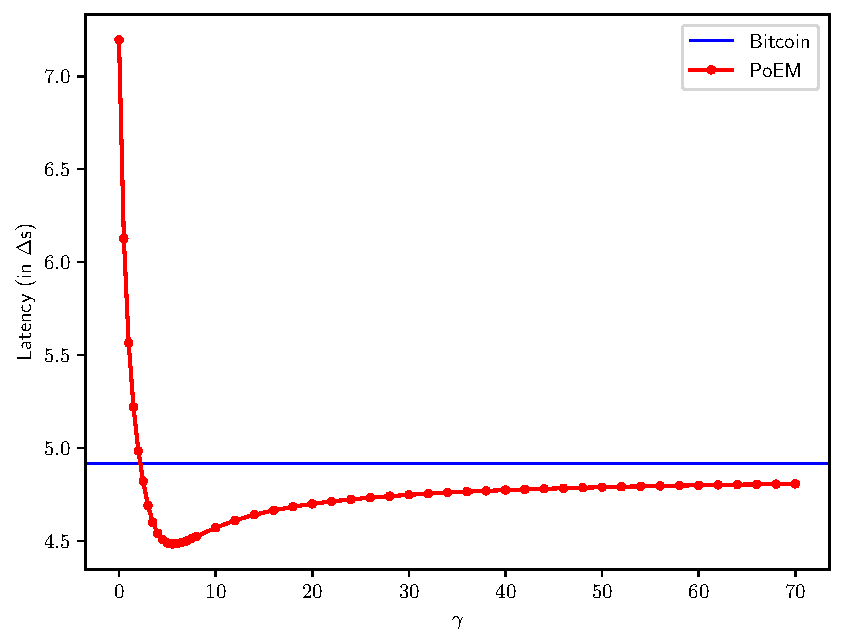
\includegraphics[width = \textwidth]{figures/gamma_latency_0.1.pdf}
    \caption{$\beta = 0.1$ and $g = 0.7$}
    \label{fig:gamma_latency_0.1}
    \end{subfigure}
    \begin{subfigure}{0.48\textwidth}
    \centering
    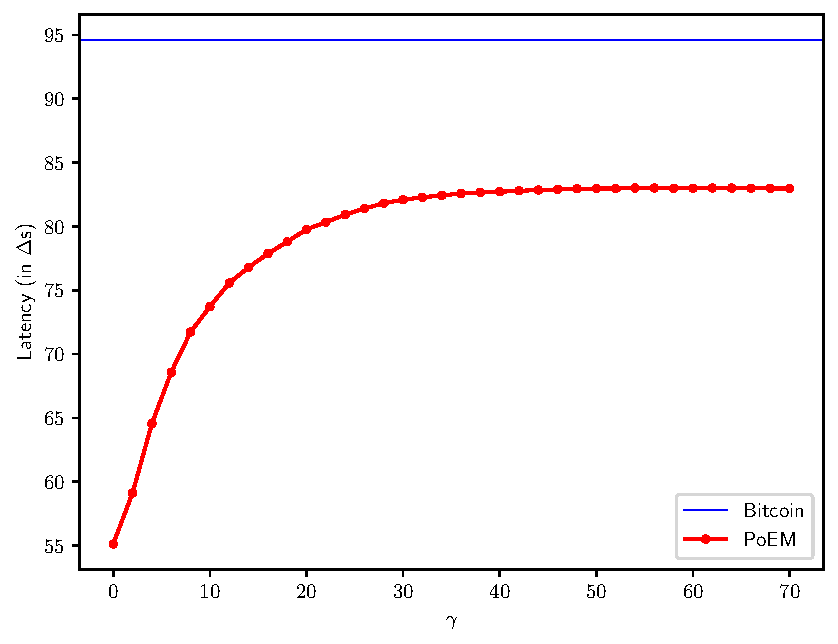
\includegraphics[width = \textwidth]{figures/gamma_latency_0.3.pdf}
    \caption{$\beta = 0.3$ and $g = 0.7$}
    \label{fig:gamma_latency_0.3}
    \end{subfigure}

  \caption{Fixing $\beta$ and $g$, we compare the latency of PoEM parameterized under different $\gamma$ values
          and the latency of Bitcoin. We observe that the plot is convex and for large $\gamma$, the latency
          converges asymptotically to a value lower than Bitcoin's latency. The results were obtained by running 100k simulations.}
    \label{fig:gamma_latency}
\end{figure}

\begin{figure}[pt]
    \centering
    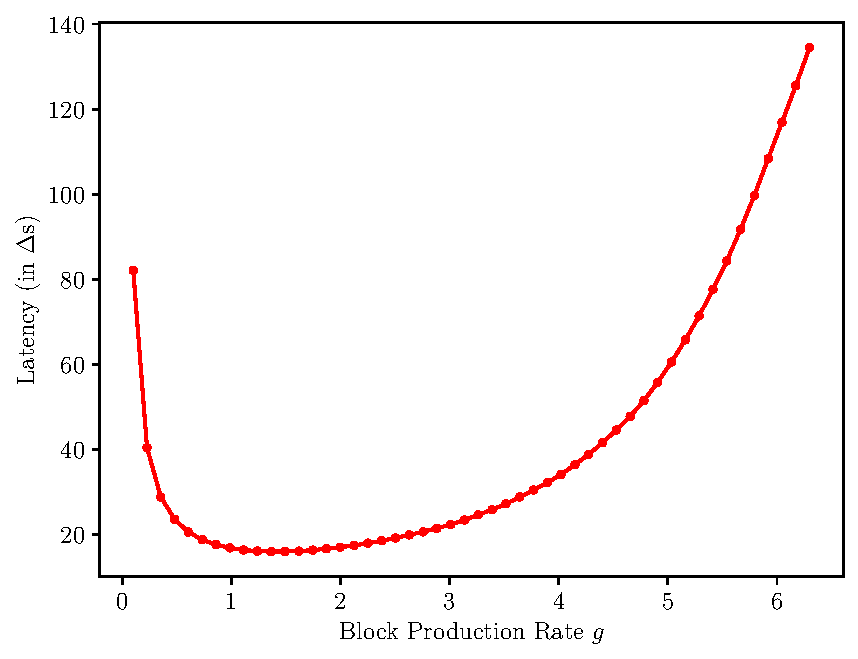
\includegraphics[width = 0.48\textwidth]{figures/g_latency.pdf}

  \caption{Fixing $\beta=0.2$ and $\gamma=0$, we plot the latency of PoEM parameterized under different block production rates $g$.
          For small block production rates, close to zero, we get high latency because blocks are produced very slow.
          For large block production rates, we get high latency because honest block create many forks, whereas the adversarial blocks
          are all chained in series. We get optimal latency somewhere in the middle.
          The results were obtained by running 100k simulations.}
    \label{fig:g_latency}
\end{figure}

We note some limitations of our experimental methodology. Firstly, the private attack has been proven optimal
for Bitcoin only, and not for PoEM, but in our experiments we have used the same attack for both protocols.
Secondly, the optimality of the private attack previously proven~\cite{eiar} is a reduction illustrating
that, for a given resilience $\beta$, if the private attack is not possible, then no attack is possible.
In our experiments, we obtain a safe confirmation parameter $k$ against the private mining attack,
but this confirmation parameter has not been shown to be safe against other attacks, even though the private
mining attack is optimal when it pertains to resilience.
Lastly, there is a discrepancy between the continuous-time model used in our experimental simulations
and the discrete-time model used in our theoretical analysis.